\documentclass[]{scrartcl}
\usepackage[a4paper,left=2cm,right=3cm,top=2cm,bottom=2cm]{geometry}
\usepackage{svg}
\usepackage{graphicx}
\usepackage[dvipsnames]{xcolor}
\usepackage{minted}
\usepackage{tcolorbox}
\usepackage[spanish]{babel}
\usepackage{mdframed}
\usepackage{epigraph}


\tcbuselibrary{minted}
\tcbuselibrary{breakable}

\definecolor{bashcodebg}{rgb}{0.85,0.85,0.85}

\newtcolorbox{notebox}{colback=SpringGreen!15!white,
colframe=SpringGreen!50!black}

\newtcolorbox{importantbox}{colback=RubineRed!25!white,colframe=RubineRed!75!black}

\newtcolorbox[auto counter]{exbox}[1][]{%
colback=red!5!white,colframe=red!75!black,
fonttitle=\bfseries,
title=Ejercicio \thetcbcounter: , #1}

\newtcblisting[auto counter]{cbox}[2][]{%
listing engine=minted,
minted language=c,
minted style=friendly,
minted options={mathescape,autogobble, framesep},
colback=TealBlue!5!white,colframe=TealBlue!75!black,
fonttitle=\bfseries,
listing only,
title=Snippet \thetcbcounter: #2, #1}

\newminted[ccode]{c}{
  style=friendly,
  linenos=false,
  autogobble,
  fontsize=\footnotesize,
  bgcolor=gray!5,
  framesep=2mm,
  baselinestretch=1.2 % Adjust line height if needed
}

\newtcblisting[auto counter]{bashbox}[1][]{%
listing engine=minted,
minted language=bash,
minted style=friendly,
minted options={mathescape,autogobble, framesep},
colback=bashcodebg,
colframe=black!70,
fonttitle=\bfseries,
listing only,
#1}

\newtcbinputlisting[]{\bashinput}[2][]{%
listing file={#2},
listing engine=minted,
minted language=bash,
minted style=friendly,
minted options={autogobble, framesep},
colback=bashcodebg,
colframe=black!70,
fonttitle=\bfseries,
listing only,
#1}

\usepackage{colortbl} % para /color
\usepackage{hyperref} % Necesario para \url y \href
\usepackage{caption} % Para usar captionof
\captionsetup{labelformat=empty, hypcap=false}

\hypersetup{
    colorlinks=true,
    linkcolor=CadetBlue,
    filecolor=CadetBlue,      
    urlcolor=CadetBlue,
    }

\newcommand{\hl}[1]{\textcolor{magenta}{\textbf{\texttt{#1}}}}

%opening
\title{Guía de C}
\subtitle{Arquitectura y Organización del Computador}
\date{}
\begin{document}


\maketitle

\section*{Introducción}
\subsection*{¿Por qué queremos aprender C?}

\begin{itemize}
  \item C es de bajo nivel, ideal para \textbf{system programming}
  \item C es \textbf{pequeño} en comparación con otros lenguajes de programación, 
  \item C permite hacer uso de los recursos subyacentes de manera mucho más sencilla.
\end{itemize}

Es un lenguaje compilado que corre directamente en el sistema host y permite manipulación directa de memoria. 
Es un lenguaje de programación de propósito general, que ha sido ampliamente utilizado en sistemas operativos, compiladores, interpretes, etc.

\subsubsection*{Puntos fuertes:}
\begin{itemize}
  \item \textbf{Eficiencia}. Las abstracciones que C permite están fuertemente arraigadas a los tipos de datos y operaciones que ofrecen las computadoras convencionales.\footnote{\url{https://dl.acm.org/doi/abs/10.1145/154766.155580}}
  \item \textbf{Portabilidad}. Teniendo ciertas precauciones, C es un lenguaje portable, lo que significa que el código fuente puede ser compilado en diferentes arquitecturas.
  \item \textbf{Ampliamente utilizado} en sistemas operativos, compiladores, interpretes, etc.
  \item Permite manipulación directa de \textbf{memoria}, lo que lo hace ideal para tareas de bajo nivel.
  \item Tiene una estructura \textbf{simple y clara}. 
\end{itemize}

\subsubsection*{Puntos débiles:}

\begin{itemize}
\item C es permisivo con las operaciones que se pueden realizar, por lo que se asume que aquel que programa \textit{sabe lo que está haciendo}.
\item Al ser un lenguaje que carece de verificación de errores automáticos (como \textit{index out of array} o \textit{null pointer reference}), los programas son más propensos a errores.
\item Los programas en C pueden ser difíciles de entender, ya que el código permite ser muy obtuso en su escritura. De hecho, existe una competencia llamada ``Obfuscated C Code Contest'' que premia al código más difícil de entender \footnote{Ver, por ejemplo: {\url{https://github.com/ioccc-src/winner/blob/master/1986/bright/bright.orig.c}}}
\item Los programas en C pueden ser más difíciles de mantener. Esto se asocia estrechamente con el ítem anterior.
\end{itemize}

\section*{Recomendaciones para usar esta guía}

Para que puedan afianzar de manera correcta los conceptos, es importante que sigan las recomendaciones que se detallan a continuación.

\begin{itemize}
  \item Empiecen con un \textbf{directorio completamente vacío}. Inicialicen un repositorio de git y hagan un commit de un archivo \texttt{.gitginore} que puede ser como \url{https://github.com/github/gitignore/blob/main/C.gitignore}
  \item \textbf{No copien y peguen el código}. Tipeenlo ustedes. Esto indefectiblemente introducirá errores y eso es \textbf{bueno}. Familiarizarse con los mensajes de error es parte fundamental del proceso de aprendizaje.
  \item Lean los mensajes de error atentamente. En la mayoría de los casos, el mensaje indica exactamente donde está el error y qué es lo que está mal.
  \item No se queden sólo con los ejemplos. Experimenten con el código, cambien cosas, rómpanlo y vean los mensajes de error.
  
\end{itemize}

El aprendizaje de un lenguaje rara vez es lineal. Es un proceso iterativo y es normal que haya que volver atrás para entender algo. Esperamos que esta guía les sirva para aprender los rudimentos de C y que puedan usarlo en de manera efectiva en la materia y en sus proyectos. Si tienen consultas, no duden en preguntar. Si les parece que existe un error o que algo se puede explicar mejor, no duden en hacérnoslo saber.

Ahora sí, ¡a programar!

\newpage

\section*{Hola Orga!}
\epigraph{\textit{- What's in the box? \newline - Pain.}}

Vaya, parece que tenemos un programa en C que nos saluda. Veamos que hace.

\begin{cbox}[unbreakable]{Hola Orga!}
  #include <stdio.h>             // Incluye la biblioteca stdio.h
  
  int main() {                   // main es el punto de entrada
      printf("Hola Orga!\n");    // imprime en pantalla
      return 0;                  // devuelve un 0 al SO
  }
\end{cbox}

Este primer código en C escribe en pantalla el texto \texttt{Hola, Orga!} en la consola y termina. Hace uso de la función \hl{printf} de la biblioteca estándar de C que imprime en pantalla. 
La función \hl{main} es el punto de entrada de cualquier programa en C y devuelve un valor al sistema operativo. Notar que devuelve un tipo \hl{int}.

Lo primero que encontramos es un \hl{\#include <stdio.h>}. \hl{\#include} es una directiva de pre-procesador (porque empieza con \hl{\#} que agrega las declaraciones al comienzo del archivo (funciona como un \textit{copy paste}).
En particular, el archivo \texttt{stdio.h} es un \textit{header file} o encabezado que se encuentra en un directorio estándar del sistema y contiene declaraciones de funciones que interactúan con entrada/salida, como lo es \hl{printf}. 

Como resumen llevémonos los siguientes conceptos básicos de un programa en C:
\begin{itemize}
\item Todo programa en C tiene una función \hl{main()}, la cual es la primer función que se ejecuta al correr un binario.
\item Todo programa en C (todo programa en realidad) devuelve un valor al sistema operativo. En este caso, el valor 0 indica que el programa terminó correctamente.
\item Las funciones en C se declaran con el tipo de dato que devuelven, seguido del nombre de la función y los parámetros que recibe.
\item Los string literales en C se escriben entre comillas dobles.
\end{itemize}

Para compilar el programa anterior, se puede hacer uso de un compilador de C, como \texttt{gcc}\footnote{Para instalar el compilador y algunas utilidades, en Ubuntu, instalar el paquete \texttt{build-essential} haciendo \texttt{sudo apt install build-essential}.}. En la terminal, escribimos:
\begin{bashbox}[]
gcc -c hola.c -o hola.o
gcc hola.o -o hola
\end{bashbox}

De esta manera, el código fuente es transformado en un código objeto .o, y luego ese archivo objeto se \textit{linkea} para formar un archivo ejecutable para el sistema operativo.
Notar que no es necesario hacer un llamado a gcc dos veces, si no que se puede hacer el llamado solo con el .c y generar el binario:

\begin{bashbox}[]
gcc hola.c -o hola
\end{bashbox}

Pero en general se hace en dos pasos para separar la compilación de la generación del binario.

Ambos comandos generan un archivo con el nombre \texttt{hola}, que puede ser ejecutado desde la terminal con el comando

\begin{bashbox}[]
./hola
\end{bashbox}

En general, usaremos la extensión \texttt{.c} para los archivos fuente de C, y \texttt{.h} para los archivos de cabecera, de los cuales hablaremos más adelante. Los binarios en linux no tienen extensión.
Para compilar, usaremos algunos flags extra que nos permiten tener más información en caso de errores, como \texttt{-Wall}, \texttt{-Wextra} y \texttt{-pedantic}

\begin{bashbox}[]
gcc -Wall -Wextra -pedantic -c hola.c -o hola.o
gcc -Wall -Wextra -pedantic hola.o -o hola
\end{bashbox}

\begin{exbox}[label=ejercicio1]
  Realizar el programa que imprima en pantalla el texto \texttt{Hola, Orga!}. Compilar con todos los flags mencionados.
\end{exbox}

Para no estar escribiendo siempre los mismos comandos, se puede usar un \texttt{Makefile}. Empecemos con lo básico de \texttt{make}

\newpage


\section*{Make}
\epigraph{\textit{It’s dangerous to go alone, take this!}}

\texttt{make} es una herramienta en la cual podemos especificar cómo se compila un programa. Un archivo \texttt{Makefile} contiene reglas que le dicen a \texttt{make} cómo compilar un programa. 

Qué es make? De acuerdo a Wikipedia:

\begin{mdframed}[backgroundcolor=yellow!15]
En el contexto del desarrollo de software, Make es una herramienta de gestión de dependencias; típicamente, las que existen entre los archivos que componen el código fuente de un programa, para dirigir su recompilación o ``generación'' automáticamente. (...) La herramienta make se usa para las labores de creación de fichero ejecutable o programa, para su instalación, la limpieza de los archivos temporales en la creación del fichero, todo ello especificando unos parámetros iniciales (que deben estar en el makefile) al ejecutarlo.

Todos los Makefiles están ordenados en forma de reglas, especificando qué es lo que hay que hacer para obtener un módulo en concreto. El formato de cada una de esas reglas es el siguiente:

\begin{center}
  \begin{Verbatim}[fontshape=it]
    target: dependencias
      commandos
  \end{Verbatim}
\end{center}

En \textit{target} definimos el módulo o programa que queremos crear, después de los dos puntos y en la misma línea podemos definir qué otros módulos o programas son necesarios para crear el target. Por último, en la línea siguiente y sucesivas (el cuerpo del \textit{target}) indicamos los \textit{comandos} necesarios para llevar esto a cabo. Es muy importante que los \textit{comandos} estén separados por un tabulador del comienzo de línea (no espacios).
\end{mdframed}

Los makefiles permiten definir dependencias entre archivos (se necesita X para compilar Y) y resolverlas en caso de ser necesario. Además, \texttt{make} es una herramienta muy útil para compilar programas grandes, ya que permite compilar solo los archivos que han cambiado y no todo el programa. Esto ahorra tiempo y recursos al compilar.

Definiendo targets y dependencias, construimos las ``recetas'' para compilar binarios y ejecutar código. Vamos a crear un archivo \texttt{Makefile}\footnote{Es importante que el archivo tenga este nombre para que el comando \texttt{make} lo reconozca} para compilar el programa \texttt{hola.c} que hicimos antes. El archivo \texttt{Makefile} se ve de la siguiente manera:

\begin{bashbox}[minted language=make]
  all: hola
  
  hola: hola.o
  	gcc -Wall -Wextra -pedantic hola.o -o hola
  
  hola.o: hola.c
  	gcc -Wall -Wextra -pedantic -c hola.c -o hola.o
  
  clean:
  	rm *.o hola

  .PHONY: all clean
\end{bashbox}

Vemos que en el \texttt{Makefile} se definen una serie de targets. Hay ciertas convenciones en el uso de \texttt{Makefile} que son importantes tener en cuenta. Por ejemplo, el target \texttt{all} es el que se ejecuta por defecto si no se especifica ningún target. Al ejecutar \texttt{make} en el directorio actual, se intentará construir \texttt{all}. Por defecto, \texttt{make} supone que un \texttt{target} es un archivo en el disco. La línea \texttt{.PHONY: all clean} indica que estos targets no son archivos, sino que son simplemente comandos que se pueden ejecutar. Esos targets, al ser \texttt{.PHONY}, siempre se consideran desactualizados.
El target \texttt{clean}, por su parte, es un target especial que se usa para limpiar los archivos generados por la compilación. En este caso, se eliminan todos los archivos \texttt{.o} y el binario \texttt{hola}.

Si creamos el archivo \texttt{Makefile} en el directorio y ejecutamos el comando \texttt{make} vemos lo siguiente en la terminal:

\bashinput{snippets/make.bash}

¿Cómo se da cuenta \texttt{make} lo que tiene que ejecutar? La respuesta es que arma un \textbf{árbol de dependencias}. En este caso particular, busca el target \texttt{all} y ve que depende de \texttt{hola}. Como \texttt{hola} no se encuentra en el directorio, busca la manera de construirlo y ve que entre sus recetas tiene una para construirlo, y que depende de \texttt{hola.o}. Como \texttt{hola.o} no se encuentra en el directorio, busca la manera de construirlo y ve que su construcción depende de \texttt{hola.c}. Como \texttt{hola.c} es un archivo fuente que se encuentra en el directorio, ejecuta los comandos definidos en esa receta. Eso termina ejecutando \hl{gcc -Wall -Wextra -pedantic -c hola.c -o hola.o}. Al terminar de hacer esto, \texttt{make} empieza a volver sobre sus pasos, y entonces ahora usa ese archivo para generar el binario \texttt{hola}, ya que ahora posee sus dependencias (\texttt{hola.o}). Continúa entonces ejecutando \hl{gcc -Wall -Wextra -pedantic hola.o -o hola}. Con eso quedan satisfechas las dependencias de \texttt{all} y por lo tanto \texttt{make} termina su trabajo.

\begin{notebox}
  Los \textit{comandos} podrían ser lo que nosotros queramos, \texttt{make} es completamente agnóstico de lo que hacen. Se supone, que deben construir el \texttt{target} (por ejemplo \texttt{hola.o}), pero eso no depende de \texttt{make}. Depende exclusivamente de lo que nosotros pongamos ahí. Lo único que \texttt{make} nos pide es que pongamos el bendito tabulador al principio de la línea.
\end{notebox}

Podemos mejorar nuestro \texttt{Makefile} para que use variables. Por ejemplo, podemos definir una variable \texttt{CC} que contenga el compilador a usar y \texttt{CFLAGS} para que contenga los flags. De esta manera, si queremos cambiar de compilador o cambiar algún flag, solo tenemos que cambiar la variable y no todas las recetas.

\begin{bashbox}[minted language=make]
  CC = gcc
  CFLAGS = -Wall -Wextra -pedantic
  
  all: hola
  
  hola: hola.o
  	$(CC) $(CFLAGS) hola.o -o hola
  
  hola.o: hola.c
  	$(CC) $(CFLAGS) -c hola.c -o hola.o
  
  clean:
  	rm *.o hola

  .PHONY: all clean
\end{bashbox}

Todavía podemos mejorar más nuestro \texttt{Makefile}. Podemos usar lo que se llaman variables automáticas. Estas variables son variables que \texttt{make} define automáticamente y que contienen información sobre el target actual. Por ejemplo, \texttt{\$@} contiene el nombre del target actual, \texttt{\$<} contiene el primer prerequisito (dependencia) y \texttt{\$\^} contiene todos los prerequisitos. También podemos definir una variable \texttt{TARGET} que contenga el nombre del binario a generar. De esta manera, si queremos cambiar el nombre del binario, solo tenemos que cambiar la variable y no todas las recetas.

\bashinput[minted language=make]{snippets/make_auto.bash}

Por ahora nos vamos a conformar con este Makefile. Cuando tengamos que compilar varios archivos, veremos algunos trucos para no ser repetitivos en las recetas.

\begin{exbox}[label=ejercicio1]
  Realizar un Makefile para compilar nuestro programa de Hola Orga! De ahora en más, todos los ejemplos que veamos en la guía, deben tener un Makefile para compilar el programa.
\end{exbox}

\newpage
\section*{Tipos de datos}
\epigraph{\textit{Data is like garbage. You’d better know what you are going to do with it before you collect it.}}

C es un lenguaje de tipado estático. ¿Qué quiere decir esto? Que el tipo de dato de una variable se define en tiempo de compilación y no puede ser cambiado en tiempo de ejecución.
Esto implica que el programador debe especificar el tipo de dato de cada variable que declare. Una variable puede hacer referencia a un número entero, un número de punto flotante, un carácter, a un puntero, etc.

\subsection*{Tipos nativos del lenguaje}
Los tipos de datos (y sus modificadores) que maneja C nativamente son los siguientes:

\begin{itemize}
  \item \textbf{Enteros}: \texttt{char}, \texttt{short}, \texttt{int}, \texttt{long}, \texttt{long long}
  \item \textbf{Reales}: \texttt{float}, \texttt{double}, \texttt{long double}
  \item \textbf{Caracteres}: \texttt{char}
  \item \textbf{Punteros}: \texttt{int*}, \texttt{char*}, \texttt{void*}, etc.
  \item \textbf{Void}: \texttt{void}
  \item \textbf{Booleanos}: \texttt{bool} (no es nativo, pero se puede usar con \texttt{\#include <stdbool.h>}, desde C99)
\end{itemize}

Para tener idea de los tamaños típicos en una arquitectura de 64 bits, podemos ver la siguiente tabla:

\begin{table}[!ht]
	\centering
	\begin{tabular}{|c|c|c|}
	\hline
	\rowcolor[HTML]{9698ED}
	{\color[HTML]{333333} \textbf{Tipo}} &
	  {\color[HTML]{333333} \textbf{Bytes}} &
	  {\color[HTML]{333333} \textbf{Rango}} \\ \hline
	char          & 1 & \begin{tabular}[c]{@{}c@{}}-128 a 127\\ $-2^7$ a $2^7-1$\end{tabular}                        \\ \hline
	\begin{tabular}[c]{@{}c@{}}unsigned char\end{tabular} &
	  1 &
	  \begin{tabular}[c]{@{}c@{}}0 a 255\\ $0$ a $2^8-1$\end{tabular} \\ \hline
	short         & 2 & \begin{tabular}[c]{@{}c@{}}-32768 a 32767\\ $-2^{15}$ a $2^{15}-1$\end{tabular}             \\ \hline
	\begin{tabular}[c]{@{}c@{}}unsigned short\end{tabular} &
	  2 &
	  \begin{tabular}[c]{@{}c@{}}0 a 65535\\ $0$ a $2^{16}-1$\end{tabular} \\ \hline
	int           & 4 & \begin{tabular}[c]{@{}c@{}}-2147483648 a 2147483647\\ $-2^{31}$ a $2^{31} - 1$\end{tabular} \\ \hline
	unsigned      & 4 & \begin{tabular}[c]{@{}c@{}}0 a 4294967295\\ $0$ a $2^{32}-1$\end{tabular}                   \\ \hline
	long &
	  8 &
	  \begin{tabular}[c]{@{}c@{}}$-9.2 \times 10^{18}$ a $9.2 \times 10^{18}$\\ $-2^{63}$ a $2^{63} - 1$\end{tabular} \\ \hline
	unsigned long & 8 & \begin{tabular}[c]{@{}c@{}}$0$ a $1.84 \times 10^{19}$\\ $0$ a $2^{64}-1$\end{tabular}        \\ \hline
	\end{tabular}%
	\end{table}

¿Por qué hablamos de tamaños típicos? Porque el tamaño de los tipos de datos en C no está definido por el estándar, sino que depende de la arquitectura y del compilador. Por ejemplo, en una arquitectura de 32 bits, un \texttt{int} puede ser de 4 bytes, mientras que en una arquitectura de 64 bits, puede ser de 8 bytes.
El estándar sólo define límites mínimos para los tamaños de los tipos de datos. A continuación, se muestra un ejemplo de cómo se pueden imprimir los tamaños de los tipos de datos en C:

\begin{cbox}[]{sizeof}

  #include <stdio.h>
  
  int main() {
  	char c = 100;
  	short s = -8712;
  	int i = 123456;
  	long l = 1234567890;
  
  	printf("char(%lu): %d \n", sizeof(c),c);
  	printf("short(%lu): %d \n", sizeof(s),s);
  	printf("int(%lu): %d \n", sizeof(i),i);
  	printf("long(%lu): %ld \n", sizeof(l),l);
  
  	return 0;
  }

\end{cbox}

Este código permite imprimir por pantalla los tamaños de algunos tipos de datos. Para ello disponemos del operador \hl{sizeof()} que devuelve el tamaño en bytes de un tipo de datos o de una variable. Este operador es muy útil para saber cuánta memoria ocupa un tipo de dato en particular. Se resuelve en tiempo de compilación.

Además, este código usa \hl{printf} de manera que se pueden observar algunas cosas:
\begin{itemize}
  \item El uso de \hl{printf} con el modificador \hl{\%lu} (\texttt{long unsigned}) para imprimir el tamaño de los tipos de datos.
  \item El uso de \hl{\%d} para imprimir un \texttt{char} y un \texttt{short}, y \hl{\%ld} para imprimir un \texttt{long}.
  \item El orden de los argumentos de \hl{printf}: primero se pone el string (con los correspondientes \textit{especificadores de conversión}) y luego las variables a imprimir, en el orden en que aparecen.\footnote{Para más información sobre los especificadores de conversión de \texttt{printf}, ver \url{https://en.cppreference.com/w/c/io/fprintf}}
\end{itemize}

\begin{exbox}[label=ejercicio2]
  Realizar un programa que imprima por pantalla todos los tamaños de los tipos de datos (con sus modificadores) vistos hasta el momento. Mirar atentamente \href{https://en.cppreference.com/w/c/io/fprintf}{la tabla de especificadores de conversión} y los \texttt{length modifiers} para saber cómo imprimir los distintos tipos de datos. Traten de fixear todos los warnings que les tire el compilador.
\end{exbox}

\subsection*{Enteros de ancho fijo}

Varias veces podemos olvidarnos del tamaño de los tipos de datos al programar, e incluso cuál es el rango de valores que puede representar un tipo en particular. Pero muchas veces, no saber esto nos puede traer problemas. Por ejemplo, si estamos programando un sistema embebido y necesitamos que un entero sea de 16 bits, pero no sabemos si \hl{int} es de 16 bits o de 32 bits, podemos tener problemas.
Para no generar confusiones, existe una biblioteca llamada \hl{stdint.h} que define nuevos tipos de datos que resuelven la ambigüedad de los tamaños.

\begin{table}[!ht]
    \centering
    \begin{tabular}{|l|l|l|l|l|}
    \hline
        ~ & 8 bits/1 byte & 16 bits/2 bytes & 32 bits/4 bytes & 64 bits/8 bytes \\ \hline
        Signed & \texttt{int8\_t} & \texttt{int16\_t} & \texttt{int32\_t} & \texttt{int64\_t} \\ \hline
        Unsigned & \texttt{uint8\_t} & \texttt{uint16\_t} & \texttt{uint32\_t} & \texttt{uint64\_t} \\ \hline
    \end{tabular}
\end{table}

Más información sobre los tipos de datos de ancho fijo en \url{https://en.cppreference.com/w/c/types/integer}.
\begin{exbox}[label=ejercicio3]
  Realizar un programa que imprima por pantalla los tamaños de los tipos de datos de ancho fijo de la biblioteca \texttt{stdint.h}.
\end{exbox}

\subsubsection*{Constantes enteras}

Las constantes en C se usan para representar valores directamente en el código. Se pueden escribir de diferentes maneras, dependiendo del tipo de dato que queramos representar: \textbf{decimal}, \textbf{octal} o \textbf{hexadecimal}.

\begin{itemize}
  \item \textbf{Decimal:} se escriben como números enteros, por ejemplo: \texttt{1234}
  \item \textbf{Octal:} se escriben con un 0 al principio, por ejemplo: \texttt{01234}
  \item \textbf{Hexadecimal:} se escriben con un \texttt{0x} o \texttt{0X} al principio, por ejemplo: \texttt{0x1234}
\end{itemize}

Los literales enteros en C son de tipo \hl{int} por defecto, pero se pueden especificar otros tipos de datos usando sufijos. Por ejemplo, para especificar un literal de tipo \hl{long} se puede usar el sufijo \hl{l} o \hl{L}, y para especificar un literal de tipo \hl{unsigned} se puede usar el sufijo \hl{u} o \hl{U}. También se pueden combinar los sufijos, por ejemplo: \hl{1234UL} es un literal de tipo \hl{unsigned long}.

\begin{cbox}{sufijos en literales enteros}
  unsigned int ui = 71U;
  signed long int sli = 9223372036854775807L;
  unsigned long long int ui = 18446744073709551615ULL;
\end{cbox}

Más información sobre los literales en C se puede encontrar en \url{https://en.cppreference.com/w/c/language/integer_constant}.
\begin{importantbox}
  \textbf{Importante:} En C, los literales enteros son de tipo \texttt{int} por defecto.
\end{importantbox}

\subsection*{Números en punto flotante}

Los números en punto flotante son aquellos que tienen una parte decimal. En C, los números en punto flotante se representan con los tipos \hl{float}, \hl{double} y \hl{long double}. La diferencia entre ellos es el tamaño y la precisión. El tipo \hl{float} ocupa 4 bytes y tiene una precisión de 6-7 dígitos decimales, el tipo \hl{double} ocupa 8 bytes y tiene una precisión de 15-16 dígitos decimales, y el tipo \hl{long double} ocupa 10 bytes (o más) y tiene una precisión de 18-19 dígitos decimales.

\subsubsection*{Constantes en punto flotante}

Las constantes en punto flotante se escriben como números decimales, por ejemplo: \hl{3.14} o \hl{2.71828}. También se pueden escribir en notación científica, por ejemplo: \hl{1.23e4} (que equivale a \hl{12300}) o \hl{1.23E4}.

Los literales en punto flotante son de tipo \hl{double} por defecto, pero se pueden especificar otros tipos de datos usando sufijos. Por ejemplo, para especificar un literal de tipo \hl{float} se puede usar el sufijo \hl{f} o \hl{F}, y para especificar un literal de tipo \hl{long double} se puede usar el sufijo \hl{l} o \hl{L}. 

\begin{cbox}{sufijos en literales en punto flotante}
  10.0   /* type double */
  10.0F  /* type float */
  10.0L  /* type long double */
\end{cbox}


\subsubsection*{const}

En C, se puede declarar una variable como \hl{const} para indicar que su valor no puede ser modificado después de su inicialización. Esto es útil para definir constantes que no deben cambiar durante la ejecución del programa. Por ejemplo:

\begin{cbox}{const}
  const int MAX = 100;
  const float PI = 3.14159;
  const int i = 1; // const-qualified int
  i = 2;           // error: i is const-qualified
\end{cbox}

\subsection*{Conversiones de tipos}
Dado una variable en C, puedo realizar una conversion de tipos de manera manual denominada \textit{casting}. Lo que permite el casting (o \textit{casteo}, como se le suele decir), es reinterpretar un valor de cierto tipo como otro.

Veamos un programa un poco más avanzado que incorpora operaciones de casteo explícito:
\begin{cbox}[]{Casting}

  #include <stdio.h>
 
  int main() {
    int mensaje_secreto[] = {116, 104, 101, 32, 103, 105, 102, 116, 32, 111, 
    102, 32, 119, 111, 114, 100, 115, 32, 105, 115, 32, 116, 104, 101, 32, 
    103, 105, 102, 116, 32, 111, 102, 32, 100, 101, 99, 101, 112, 116, 105, 
    111, 110, 32, 97, 110, 100, 32, 105, 108, 108, 117, 115, 105, 111, 110};

    size_t length = sizeof(mensaje_secreto) / sizeof(int);
    char decoded[length];
    
    for (int i = 0; i < length; i++) {
      decoded[i] = (char) (mensaje_secreto[i]); // casting de int a char
    }
  
    for (int i = 0; i < length; i++) {
      printf("%c", decoded[i]);
    }
  }

\end{cbox}

En este código, se realizan casts de \texttt{int} a \texttt{char} para poder imprimir el mensaje secreto. El cast se realiza con el operador \texttt{(tipo)}. 

La sintaxis general para hacer un casting es:

\begin{bashbox}[]
  (type) expression
\end{bashbox}

Este tipo de cast se denomina explícito, ya que el programador está indicando explícitamente que quiere que la variable sea interpretada como otro tipo. Existen otros tipos de cast, como el cast implícito, que se realiza automáticamente por el compilador. Las conversiones implícitas, suceden automáticamente en expresiones a medida que son requeridas. Las reglas son \textit{bastante complejas}, pero en general, el compilador intenta hacer la conversión más segura posible. Por ejemplo, si se suma un \texttt{int} y un \texttt{float}, el compilador convertirá el \texttt{int} a \texttt{float} antes de realizar la suma. Esto se denomina promoción de tipo. Para más información ver \url{https://en.cppreference.com/w/c/language/conversion}.

Los cast son una herramienta poderosa, pero también peligrosa, ya que se pueden perder datos si no se hace correctamente. Por ejemplo, si se castea un \texttt{int} a un \texttt{char} y el valor del \texttt{int} es mayor a 127, se perderán bits de información.\footnote{Sólo si el char es \texttt{signed} que es lo típico. Si es \texttt{unsigned}, el rango es de 0 a 255. Ah sí, el tipo \texttt{char} ``a secas'' puede ser \texttt{signed} o \texttt{unsigned} dependiendo de la implementación.}

Dependiendo del cast, pueden pasar dos cosas: 
\begin{itemize}
  \item se reinterpretan el tipo de datos, sin modificar la representación binaria 
  
  \hl{int* i = (int*) un\_int;}
  
  \item se modifica la representación binaria del dato, por ejemplo en 
  
  \hl{int i = (int) un\_float;}
\end{itemize}

En general, si tenemos activados los warnings del compilador, vamos a tener un warning si se realiza un cast implícito que pueda perder información. Si realizamos un cast explícito, el compilador no nos va a avisar si estamos perdiendo información, ya que asume que el programador sabe lo que está haciendo.

\begin{exbox}
  Realizar un programa que imprima el valor de \texttt{0.1} como \texttt{float} y como \texttt{double}. Luego, realizar un cast de \texttt{float} a \texttt{int} y de \texttt{double} a \texttt{int}. ¿Qué sucede?
\end{exbox}

\begin{exbox}
  Compilar y ejecutar el programa del mensaje secreto. ¿Qué mensaje se imprime? ¿Por qué les parece que \texttt{length} se calcula de esa manera? ¿Qué pasaría si el mensaje secreto tuviera un tamaño distinto? ¿Por qué se usa \texttt{size\_t} para calcular el tamaño del mensaje secreto? Ver \url{https://en.cppreference.com/w/c/types/size_t} para más información.
\end{exbox}

\newpage

\section*{Operadores}
\epigraph{\textit{Language itself is an operator on the mind, shaping what we see and how we interpret the world.}}

En C, disponemos de varios operadores que nos permiten realizar operaciones aritméticas, lógicas, de comparación, etc. A continuación, se muestra una tabla con los operadores más comunes en C:

  \begin{table}[H]
    \centering
    \resizebox{0.6\textwidth}{!}  & aritméticos            \\ \hline
    \texttt{<,<=,>,>=,==,!=}  & comparación            \\ \hline
    \texttt{\&\&,||,!}   & lógicos                \\ \hline
    \texttt{\&,\textless\textless,\textgreater\textgreater,|,$\sim$,\^}  & binarios               \\ \hline
    \texttt{=,+=,-=,*=,/=,\%=}  & asignación             \\ \hline
    \texttt{?:}  & condicional            \\ \hline
    \end{tabular}%
    }
  \end{table}

Se encuentran agrupados por tipo de operación, no por precedencia. La precedencia de los operadores en C se puede ver en la siguiente tabla: \href{https://en.cppreference.com/w/c/language/operator_precedence}{Tabla de precedencia de operadores en C}

Asimismo, en esa tabla podemos observar la asociatividad de los operadores. Por ejemplo, es equivalente escribir \hl{a * b / c} que \hl{(a * b) / c}, ya que el operador \hl{*} y \hl{/} tienen asociatividad de izquierda a derecha.

Asimismo, operaciones como \hl{a = b = c} son posibles en C porque el operador de asignación tiene asociatividad de derecha a izquierda.

Algunas cosas a tener en cuenta:
\begin{itemize}
  \item \hl{++i} incrementa \hl{i} y luego devuelve el valor de \hl{i}.
  \item \hl{i++} devuelve el valor de \hl{i} y luego incrementa \hl{i}.
  \item \hl{a = b = c = 0} asigna 0 a las variables \hl{a}, \hl{b} y \hl{c}.
  \item \hl{a = b = c} asigna el valor de \hl{c} a \hl{a} y \hl{b}.
  \item los operadores de comparación devuelven 1 si la condición es verdadera y 0 si es falsa.
  \item un entero es considerado verdadero si es distinto de 0.
\end{itemize}

\begin{exbox}[]
  Realizar un programa que imprima por pantalla el resultado de las siguientes operaciones:
  \begin{itemize}
    \item \texttt{a = 5, b = 3, c = 2, d = 1}
    \item \texttt{a + b * c / d}
    \item \texttt{a\space\space\% b}
    \item \texttt{a == b, a != b}
    \item \texttt{a \& b, a | b}
    \item \texttt{$\sim$a}
    \item \texttt{a \&\& b, a || b}
    \item \texttt{a \textless\textless \space1}
    \item \texttt{a \textgreater\textgreater \space1}
    \item \texttt{a += b, a -= b, a *= b, a /= b, a \%= b}
  \end{itemize}
  \textbf{Importante:} Interpretar los resultados de las operaciones y ver si coinciden con lo esperado. Para imprimir los valores de las operaciones binarias, usar \texttt{\%x} o también \texttt{\%X} en \texttt{printf}.
\end{exbox}

\begin{exbox}[label=ejercicio5]
  Realizar un programa que muestre la diferencia entre \texttt{++i} y \texttt{i++}.
\end{exbox}

Veamos ahora algunas manipulaciones de bits las cuales tienen especial relevancia en la materia: \textbf{shifting} y \textbf{máscaras}.

\subsection*{Shifting}

Repasemos antes las operaciones de shift a izquierda y derecha. Estas operaciones son muy utilizadas en C para manipular bits.

Algunas limitaciones a tener en cuenta en las operaciones de shifteo:
\begin{itemize}
  \item En \hl{a \textless\textless \space b}, los bits que se desplazan a la izquierda se pierden.
  \item En \hl{a \textgreater\textgreater \space b}, los bits que se desplazan a la derecha se pierden.
  \item En \hl{a \textless\textless \space b} y en \hl{a \textgreater\textgreater \space b}, el tipo de \hl{b} se promociona al tipo de \texttt{a}.
  \item \hl{b} debe estar entre 0 y el tamaño en bits del tipo de \hl{a} menos 1. Por ejemplo, si \hl{a} es un \hl{uint32\_t}, \hl{b} puede valer entre 0 y 31. En otro caso, el comportamiento es indefinido.
  \item Si \hl{b} es negativo, el comportamiento es indefinido.
\end{itemize}

\begin{center}
  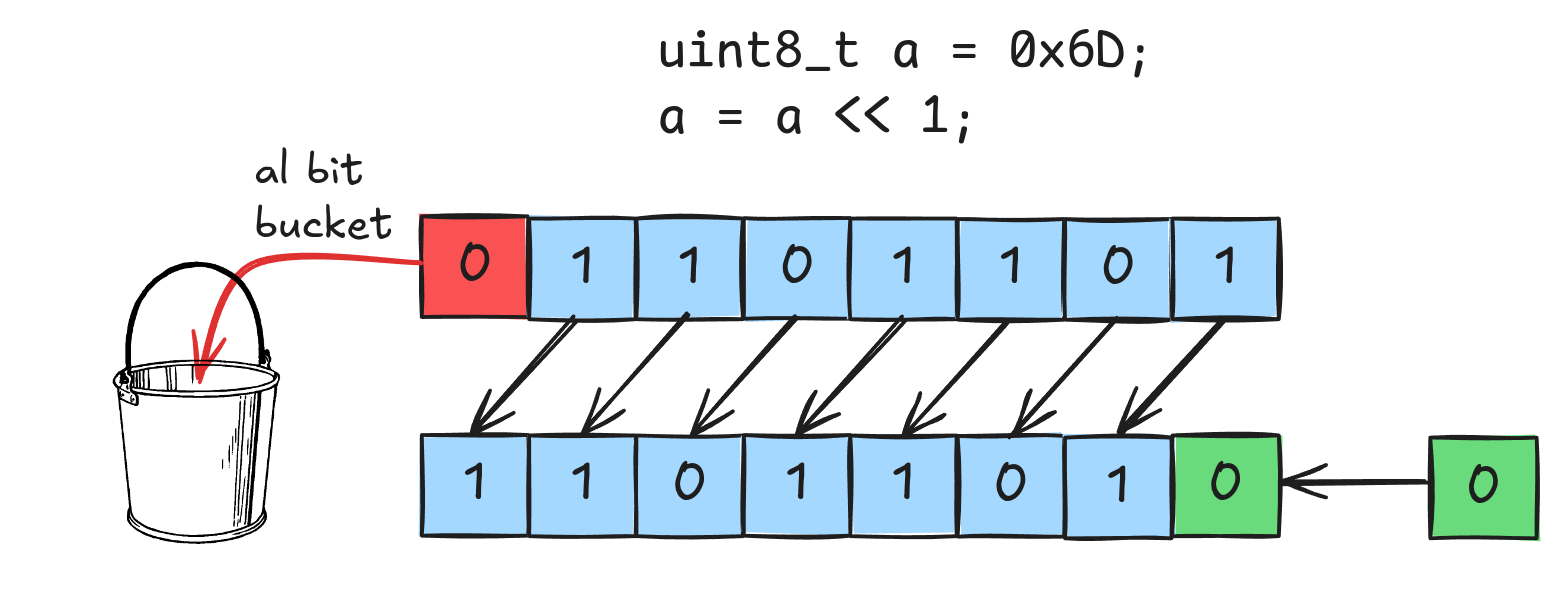
\includegraphics[scale=0.4]{./img/shift_left.png}  
  \captionof{table}{Shifteo a izquierda}
  \label{fig:Shift_left}
\end{center}

En relación al shift a derecha:
\begin{itemize}
  \item Cuando shifteamos a derecha un entero con signo, se realiza un shifteo aritmético, es decir, se rellena con el bit de signo.\footnote{En realidad, en este caso el comportamiento es \textit{implementation defined} según el estándar, pero en la práctica, en la mayoría de las arquitecturas, se realiza un shifteo aritmético.}
  \item Cuando shifteamos a derecha un entero sin signo, se realiza un shifteo lógico, es decir, se rellena con ceros a la izquierda.
\end{itemize}

\begin{center}
  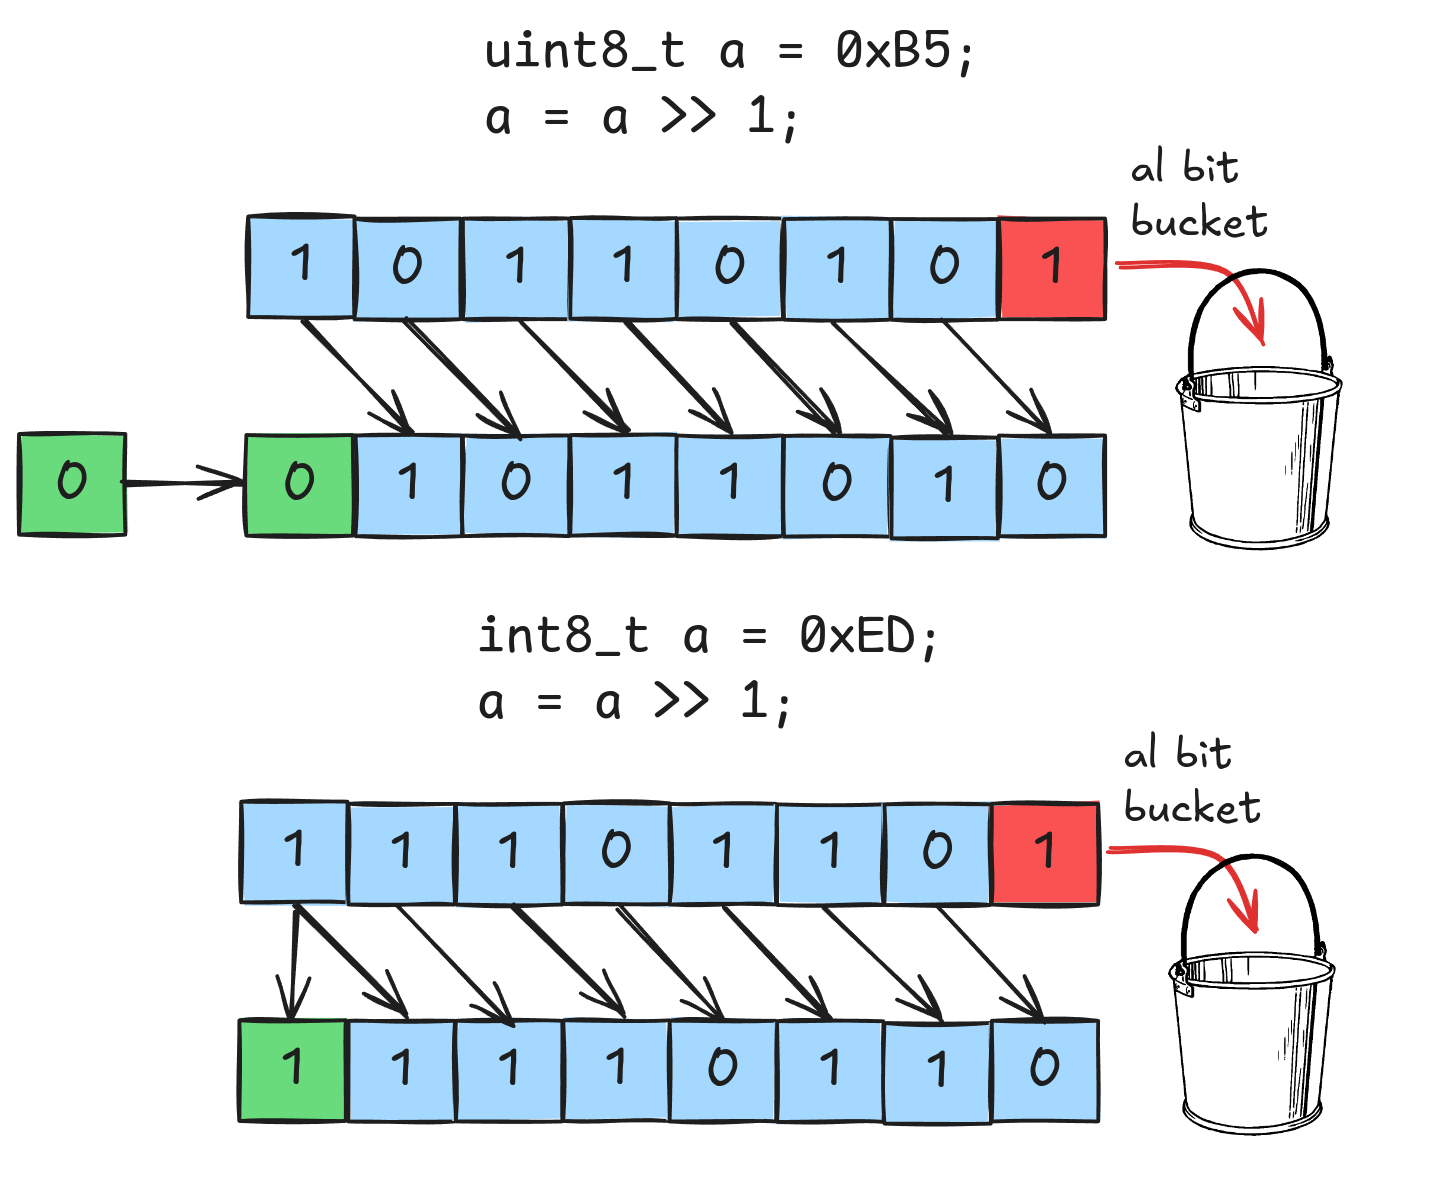
\includegraphics[scale=0.5]{./img/shift_right.png}  
  \captionof{table}{Shifteo a derecha}
  \label{fig:Shift_right}
\end{center}

\subsection*{Máscaras}

La operación de máscara es una operación muy común en C. Consiste en aplicar una operación binaria de AND u OR bit a bit entre dos números, de manera de afectar ciertos bits de una \textit{palabra}\footnote{Nos referimos a \textit{palabra} de manera genérica para hablar de una secuencia de bits que tenga sentido tratar como una unidad, por ejemplo 32-bits} con 0 o con 1, dejando el resto de los bits intactos. Por eso se llama máscara, porque enmascaramos a los bits que no queremos modificar.

\begin{center}
  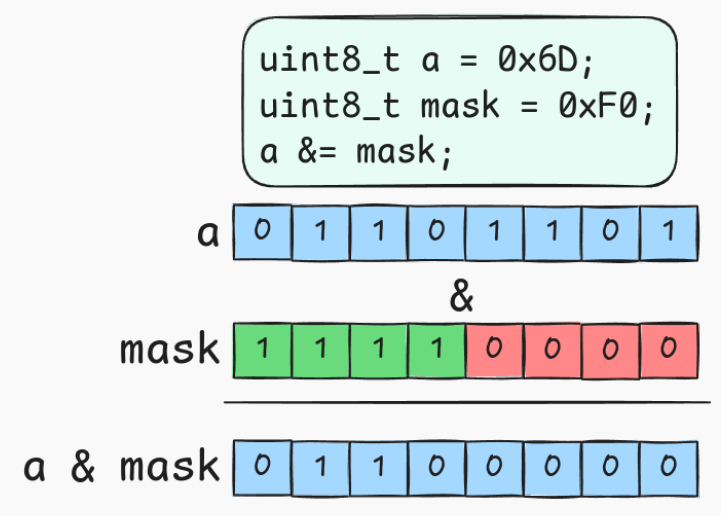
\includegraphics[scale=0.3]{./img/mask.png}
  \captionof{table}{Operación de máscara}
  \label{fig:masking}
\end{center}

Poner un bit en 1 en una palabra se llama \textit{set} y poner un bit en 0 se llama \textit{clear}. Para \textit{setear} un bit, se hace un OR bit a bit con 1, y para \textit{clearear} un bit, se hace un AND bit a bit con 0.
Por ejemplo, si queremos combinar dos palabras de 8 bits, de manera que algunos bits sean de una palabra y el resto de la otra, podemos hacer dicha mezcla de la siguiente manera:

\begin{center}
  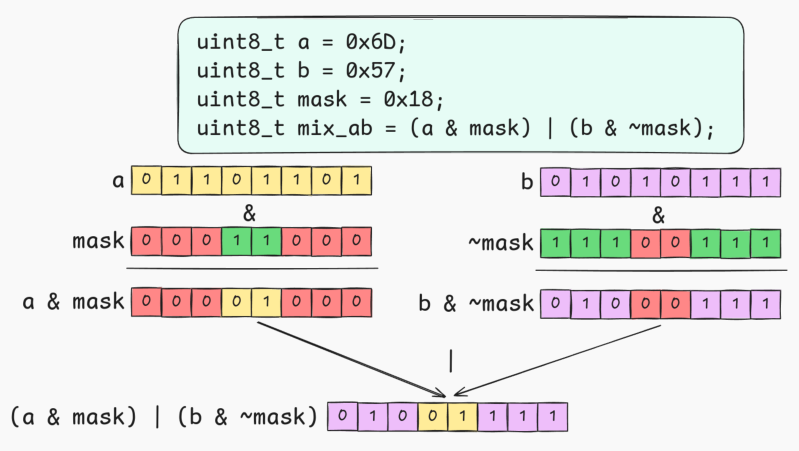
\includegraphics[scale=0.4]{./img/mask_multiple.png}
  \captionof{table}{Mezcla de palabras de 8 bits}
  \label{fig:masking_mix}
\end{center}

Las operaciones de máscara se utilizan en el paradigma de procesamiento SIMD (Single Instruction Multiple Data) para procesar varios datos al mismo tiempo. En este paradigma, se utilizan registros de 128 bits o más para procesar varios datos al mismo tiempo. Las operaciones de máscara permiten seleccionar qué datos se dejan pasar y cuáles no, lo que permite hacer mezclas de datos de manera eficiente.
\begin{exbox}
  Realizar un programa que compare si los 3 bits más altos de una palabra de 32 bits son iguales a los 3 bits más bajos de otra palabra de 32 bits. Si son iguales, informarlo por pantalla. 
\end{exbox}

\newpage
\section*{Estructuras de control}

\epigraph{\textit{I believe in creative control. No matter what anyone makes, they should have control over it.}}

En las siguientes estructuras de control, usaremos una \hl{condition} para decidir si se ejecuta un bloque de código o no. La \hl{condition} puede ser cualquier expresión que devuelva un valor entero. Esto es algo sumamente utilizado en C, ya que el valor 0 es considerado falso y cualquier otro valor es considerado verdadero. Si bien se dispone de tipos booleanos desde C99, el uso de enteros para representar verdadero o falso es una práctica extremadamente común y aceptada idiomáticamente en C.

\subsubsection*{If-else}

Ejemplo de uso de estructura \texttt{if-else}:

\begin{cbox}[]{if-else}
  #include <stdio.h>
  
  int main() {
    int a = 5;
    if (a % 2) {
      printf("a es impar\n");
    } else {
      printf("a es par\n");
    }
    return 0;
  }
\end{cbox}

\subsubsection*{ciclos}

Un ciclo \hl{while} se ejecuta mientras la condición sea verdadera. La sintaxis de un ciclo \texttt{while} es la siguiente:

\begin{cbox}[]{while}
  while (condition) {
    // código
  }
\end{cbox}

Analicemos el siguiente ejemplo:

\begin{cbox}[]{while}
  #include <stdio.h>

  int main() {
    int i = 10;
  
    while(i--){
      printf("i = %d\n",i); // imprime o no el 0?
    }
  }

\end{cbox}

\begin{notebox}
  \textbf{Nota:} para responder la pregunta, recordar como funciona el operador post-decremento.
\end{notebox}

La sintaxis de un ciclo for es la siguiente:

\begin{cbox}[]{for}
  for (initialization; condition; update) {
    // código
  }
\end{cbox}

La \hl{initilization} se ejecuta una sola vez al principio del ciclo, mientras que \hl{condition} se evalúa en cada iteración y si es verdadera se ejecuta el bloque de código, y \hl{update} se ejecuta al final de cada iteración.

\begin{cbox}[]{for example (pun intended)}
  #include <stdio.h>
  
  int main() {
    for (int i = 0; i < 10; i++) {
      printf("%d\n", i);
    }
    return 0;
  }
\end{cbox}

Notar como podemos declarar variables en la inicialización del ciclo \hl{for}. El scope de dichas variables es local al ciclo.

Todo ciclo puede ser interrumpido con la sentencia \hl{break}, que termina el ciclo en el que se encuentra, y \hl{continue}, que saltea el resto del bloque de código y pasa a la siguiente iteración.
Generalmente, si sabemos la cantidad de veces que vamos a iterar, usamos un ciclo \hl{for}, y si no, usamos un ciclo \hl{while}. Pero es una cuestión de estilo y preferencia. Ambas estructuras se pueden usar indistintamente y se pueden reemplazar una por la otra.

\begin{exbox}[]
  Reemplazar el ciclo \hl{while} del snippet anterior por un ciclo \hl{for}.
\end{exbox}
 
Y ya que estamos con ciclos, pasemos a ver \texttt{arrays} y \texttt{strings}.

\subsection*{Arrays}
Un array es una tira contigua en memoria de elementos del mismo tipo.

\begin{cbox}[]{}
#define N 4

uint32_t a[N];
a[0] = 0;
a[1] = 20;
a[2] = 14;
a[3] = 40;

\end{cbox}

\begin{center}
  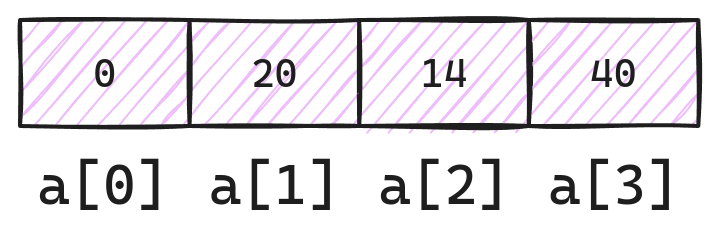
\includegraphics[scale=0.25]{./img/array.png}
  \captionof{table}{Array}
  \label{fig:array}
\end{center}

Depende de donde esté definido, un array puede estar sin inicializar. En ese caso, los valores de los elementos del array son basura. Veamos como se inicializa típicamente un array:

\begin{cbox}[]{}
  #define N 100

  uint32_t a[N];
  int i = 0;
  while(i < N){
    a[i] = i;
    i++;
  }
\end{cbox}

\begin{cbox}[]{}
  #define N 100

  uint32_t a[N];
  for (int i = 0; i < N; i++){
    a[i] = i;
  }
\end{cbox}

También se pueden inicializar los elementos de un array al momento de declararlo:

\begin{cbox}[]{}
#define N 4
uint32_t a[N] = {0, 20, 14, 40};
uint32_t b[] = {0, 20, 14, 40};
uint32_t c[N] = {0}; // c es {0, 0, 0, 0}
uint32_t d[] = {[1] = 20, [2] = 14, [3] = 40};
\end{cbox}


Ahora, ¿Cómo es que se guardan los valores en memoria?
Recordar que dijimos que un array es una tira contigua de elementos de un mismo tipo. Por lo tanto, los elementos de un array se guardan en memoria de manera contigua. A continuación, se muestra un ejemplo de cómo se guarda en memoria un array de 4 elementos de tipo \hl{uint32\_t}:

\begin{center}
  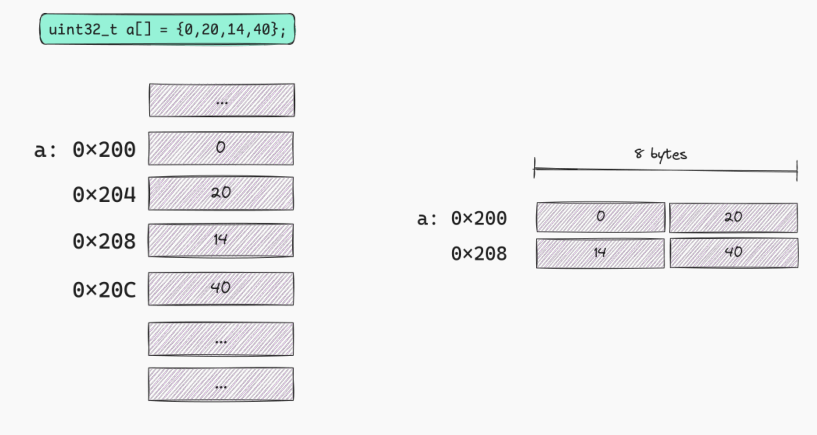
\includegraphics[scale=0.5]{./img/array_memoria.png}
  \captionof{table}{Array: Memoria}
  \label{fig:array_memoria}
\end{center}

En este ejemplo, se supone que el array se ubica en la posición de memoria \texttt{0x200}. Cada elemento del array ocupa 4 bytes, ya que es un \hl{uint32\_t}. Por lo tanto, el primer elemento del array se ubica en la posición de memoria \texttt{0x200}, el segundo en \texttt{0x204}, etc.

\begin{importantbox}
  \centering
  \textbf{No hay nada que indique dónde termina un array. Depende de nosotros como programadores saber dónde termina.}
\end{importantbox}


\subsection*{Strings}
C no contiene un tipo de dato nativo \textit{strings}, pero sí tiene un tipo \textit{char} que sirve para representar caracteres en formato \href{https://www.asciitable.com/}{ASCII}. Con este tipo, podemos definir strings como un array de caracteres.
La convención en C es que todo string termina en un carácter nulo (\hl{\textquotesingle\textbackslash0}\textquotesingle), y con esto se puede determinar el final del string. Por ejemplo, el string ``Hola!'' se define de la siguiente manera:


\begin{cbox}[]{strings}
  char s[] = "Hola!";                         // string literal
  char u[] = {'H', 'o', 'l', 'a', '!', '\0'}; // char literals
\end{cbox}

Ambas definiciones son equivalentes. La representación de un string en memoria es la siguiente:

\begin{center}
  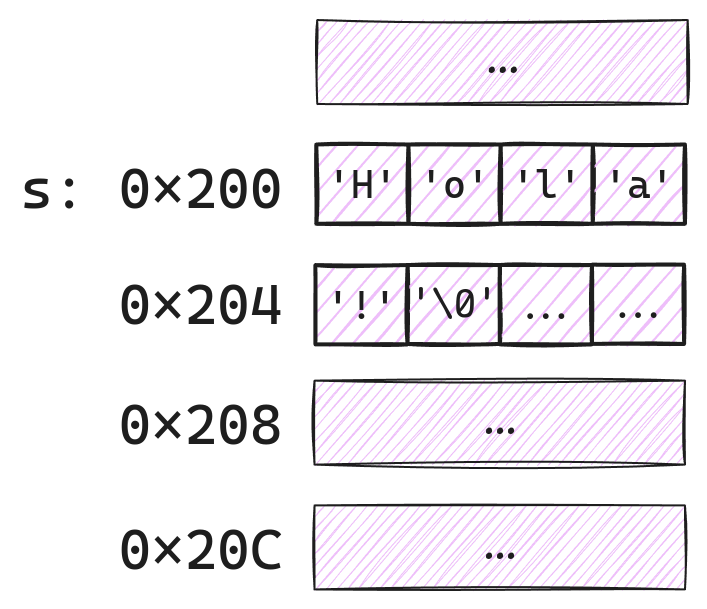
\includegraphics[scale=0.3]{./img/string_memoria.png}
  \captionof{table}{String}
  \label{fig:string}
\end{center}

Hay una sutileza en la definición de un string literal. Un string literal es un array de caracteres constante. Por lo tanto, no se puede modificar. Si se intenta modificar un string literal, el comportamiento es indefinido. Analicemos el siguiente código\footnote{Vemos que aparece un puntero a un char, lo veremos más adelante.Tomarlo simplemente como una variable que guarda la dirección de memoria de un char.}:

\begin{cbox}[]{string literal}
  int main(){
    char s[] = "Hola!"; // s es el nombre del array
    char *u = "string"; // u es un puntero a un char
    
    printf("s = %s\n", s);
    printf("u = %s\n", u);
    s[0] = 'h'; // s = "hola!"
    u[0] = 'S'; // ERROR
  }
\end{cbox}

\begin{notebox}
  \textbf{Nota:} Si se intenta modificar un string literal, el compilador no necesariamente va a tirar un error. En general, el compilador va a reservar un espacio de memoria para el string literal y va a intentar escribir en ese espacio. Si el espacio de memoria es de solo lectura, el sistema operativo va a arrojar un error de segmentación.
\end{notebox}

\begin{bashbox}
$ gcc -Wall -Wextra -pedantic strings.c -o strings
$ ./strings
s = Hola!
u = string
[1] 65377 segmentation fault (core dumped) ./strings  
\end{bashbox}

\begin{notebox}
  \textbf{Nota:} El error de segmentación (segmentation fault) es un error que ocurre cuando un programa intenta acceder a una dirección de memoria que no tiene permiso para acceder. Esto puede ocurrir por varias razones, como intentar escribir en un string literal, o intentar acceder a un puntero nulo.
\end{notebox}

%TODO: agregar funciones con strings de libc

\begin{exbox}
  Realizar un programa que rote un arreglo de números enteros a la izquierda. Por ejemplo, si el arreglo es \hl{[1, 2, 3, 4]}, el resultado debe ser \hl{[2, 3, 4, 1]}. 
\end{exbox}
\begin{exbox}
  Generalizar el ejercicio anterior para que la rotación sea un parámetro de entrada. Por ejemplo, si el arreglo es \hl{[1, 2, 3, 4]} y la rotación es 2, el resultado debe ser \hl{[3, 4, 1, 2]}.
\end{exbox}
\begin{exbox}
  Realizar un programa que tire un dado de 6 caras 60 millones de veces y cuente la cantidad de veces que salió cada número. Para esto, usar un array de 6 elementos. Luego imprimir el resultado por pantalla.
  Para tirar el dado aleatoriamente, usar la función \texttt{rand()} de la librería \texttt{stdlib.h}. Ver el ejemplo de uso provisto en \url{https://en.cppreference.com/w/c/numeric/random/rand}.
\end{exbox}

\newpage
\section*{Declaración y definición}
\epigraph{\textit{The gift of words is the gift of deception and illusion}}

Para seguir avanzando en nuestro aprendizaje de C, tenemos que hacer una distinción clara entre dos conceptos: \textit{declaración} y \textit{definición}. Veamos su definición (\textit{pun not intended}):

\textbf{Definición} se refiere al lugar en donde la variable es creada o donde se le asigna un espacio en memoria (\textit{storage}). En el caso de funciones, la definición es el lugar en donde se le asigna un procedimiento a la función.

\textbf{Declaración} se refiere a los lugares en donde la naturaleza de la variable es anunciada, pero no se le asigna un espacio en memoria.

La \textbf{declaración} especifica el tipo de una variable/función. Esta es usada por el compilador para asegurar ciertas propiedades de tipos (Por ejemplo, que dos números de tipo \hl{int} puedan ser sumados, o que el tipo que recibe una función sea el esperado). Toda variable en C debe ser declarada antes de que pueda ser usada. La forma en la que lo hacemos es escribir el tipo de la variable y su nombre.

Por otro lado, la \textbf{definición} corresponde a darle un valor concreto al identificador declarado. Para el caso de variables se le asignan valores del tipo, mientras que para funciones, se define al asignarle el procedimiento a efectuar. Tener en cuenta que en muchas situaciones, aunque no estemos explícitamente dando un valor a una variable, el compilador lo hace por nosotros, y esto representa entonces una definición. 

El lenguaje nos permite declarar y definir al mismo tiempo.

\begin{cbox}[]{}

  extern int mi_int;                   // decl

  int sumarUno(int numero);            // decl

  double sumar(double num1, double num2){ // decl y def
    return num1 + num2;
  }

  int main(){
    int i = 0;                         // decl y def
    
    char line[1000];                   // decl y def
    const double e = 2.71828182845905; // decl y def

    int count;                         // decl y def
    count = 10;                        
  }
\end{cbox}

Veamos línea por línea:
\begin{itemize}
  \item \hl{extern int mi\_int} \textbf{declara} una variable de tipo \hl{int}. Su definición puede estar en otro archivo.\footnote{Veremos el uso de la palabra clave \texttt{extern} más adelante.}
  \item \hl{int sumarUno(int numero)} \textbf{declara} una función que toma un valor de tipo \hl{int}, y devuelve \hl{int}.
  \item \hl{double sumar(double num1, double num2)} \textbf{declara} y \textbf{define} una función que toma dos valores de tipo \hl{double}, y devuelve \hl{double}.
  \item \hl{int i = 0} \textbf{declara} y \textbf{define} una variable con su tipo (\hl{int}) y nombre (\hl{i}) y la \textbf{define} con un valor concreto (\hl{0}). 
  \item \hl{char line[1000]} \textbf{declara} una variables con su tipo (\hl{char[]}) y nombre (\hl{line}) y la \textbf{define} con valores basura. 
  \item \hl{const double e = 2.71828182845905} \textbf{declara} y \textbf{define} una variable con su tipo (\hl{double}) y nombre (\hl{e}) y la \textbf{define} con un valor concreto (\hl{2.71828182845905}).
  \item \hl{int count} \textbf{declara} una variable con su tipo (\hl{int}) y nombre (\hl{count}) y la \textbf{define} con valores basura.
  \item \hl{count = 10} simplemente asigna el valor \hl{10} a la variable count. Se trata de una \textbf{asignación}. 
\end{itemize}

Hay una regla en C, llamada \textit{One Definition Rule} (ODR), que dice que:

\begin{importantbox}
  \centering
  \textbf{Una variable o función puede ser declarada múltiples veces en distintos lugares pero solo puede ser definida una vez.}
\end{importantbox}

\subsection*{Scope y duración de un identificador}

En C, un identificador es un nombre que se le da a una variable, función, estructura, etc. Un identificador tiene dos propiedades importantes: \textit{scope} y \textit{duración}.

\subsubsection*{Scope}
El \textit{scope} de un identificador es el lugar en el código donde este puede ser accedido. Este concepto es alcanzado tanto para variables como para nombres de funciones.
Los scopes pueden ser\footnote{Hay más, pero estos son los más comunes}:
\begin{itemize}
    \item \textbf{Block scope:} El identificador puede ser accedido en cualquier lugar posterior a su declaración en el mismo bloque donde se define. Para que un identificador tenga \textit{block scope}, debe ser declarado dentro de un bloque de código (por ejemplo, dentro de una función o un bucle).
    \item \textbf{File scope:} El identificador puede ser accedido en cualquier lugar posterior a su declaración dentro del mismo archivo. Para que un identificador tenga \textit{file scope}, debe ser declarado fuera de cualquier función. Se les llama también \textbf{variables globales}.
\end{itemize}

\subsection*{Duración}
La duración de una variable es el tiempo durante el cual existe. En ese tiempo, la variable tiene un espacio de memoria asignado. No quiere decir que pueda ser accedida, eso depende del scope. quiere decir que la variable tiene un espacio de memoria asignado.
Las duraciones pueden ser:
\begin{itemize}
    \item \textbf{Estática:} La variable existe durante toda la ejecución del programa. Toda variable global es estática. Se destruye cuando el programa termina.
    \item \textbf{Automática:} La variable existe durante el llamado a una función. Se destruye cuando la función termina. Esto es lo que sucede con las variables locales a una función.
    \item \textbf{Dinámica:} La variable existe durante el tiempo que se le asigna memoria. Esto es controlado por el programador. Se crea, por ejemplo, cuando se llama a la función \hl{malloc} y se destruye cuando se llama a la función \hl{free}. Lo veremos más adelante.
\end{itemize}

Toda variable local a una función tiene, por defecto, una duración \textit{automática} y un \textit{block scope}. Por otro lado, toda variable global tiene una duración \textit{estática} y un \textit{file scope}.

Además, toda variable global no inicializada explícitamente es inicializada a 0. Esto no sucede con las variables locales. Por lo tanto, si una variable local no es inicializada explícitamente, su valor es basura.

Se conoce como \textit{shadowing} a la situación en la que una variable local tiene el mismo nombre que una variable global. En este caso, la variable local "oculta" a la variable global. Esto puede llevar a confusiones y errores, por lo que se recomienda evitarlo.

Veamos un ejemplo de \textit{shadowing}:
\begin{cbox}[]{}
  #include <stdio.h>

  int i; // inicializada a 0

  void funcion() {
    int i = 1; // variable local
    printf("i = %d\n", i); // imprime 1
  }

  int main() {
    funcion();
    printf("i = %d\n", i); // imprime 0
    return 0;
  }
\end{cbox}
En este ejemplo, la variable global \hl{i} es inicializada a 0. Luego, en la función \hl{funcion}, se declara una variable local \hl{i} que es inicializada a 1. Cuando se imprime el valor de \hl{i} dentro de la función, se imprime 1. Sin embargo, cuando se imprime el valor de \hl{i} en la función \hl{main}, se imprime 0, ya que se está accediendo a la variable global.

\begin{exbox}
  Realizar un programa que declare una variable global y una variable local. Luego, imprimir el valor de ambas variables en la función \hl{main}. Luego, probar darles el mismo nombre. ¿Qué sucede? ¿Por qué? 
\end{exbox}

\newpage
\section*{Funciones}

\epigraph{\textit{Words can carry any burden we wish. All that's required is agreement and a tradition upon which to build.}}

En C, una función esta conformada por el nombre que lleva, el tipo, orden y número de parámetros que recibe y el tipo de retorno. 
La sintaxis de una función es la siguiente:

\begin{center}
  \begin{Verbatim}[fontshape=it]
  return-type function-name (parameters){
    declarations
    statements
  }	
  \end{Verbatim}
\end{center}

Las funciones pueden retornar un valor de un tipo en particular (por ejemplo, \hl{int}), o si no devuelven nada, esto se indica con el tipo especial \hl{void}. Es necesario declarar toda función antes de ser usada\footnote{Recordemos que una definición puede servir como declaración, de la misma forma que en definiciones de variables}. Asi también pueden haber múltiples declaraciones de una misma función, pero solo puede haber una única definición de la misma (ODR).

\subsection*{Pasaje de parámetros}

En C, los parámetros de una función son pasados por valor. Esto significa que se crea una copia de la variable que se pasa como argumento. Por lo tanto, si se modifica el valor de un parámetro dentro de una función, no se modifica el valor de la variable original. Veamos un ejemplo:

\begin{cbox}[]{Pasaje por valor}
  #include <stdio.h>
  
  void duplicar(int n) {
    n = n * 2;
  }
  
  int main() {
    int n = 5;
    duplicar(n);
    printf("%d\n", n); // imprime 5
    return 0;
  }
\end{cbox}

Para poder modificar el valor de una variable, se puede pasar un puntero a la función. Un puntero es una variable que guarda la dirección de memoria de otra variable. Lo veremos más adelante.

Entonces recordar:

\begin{importantbox}
  \centering
  \textbf{Los parámetros de una función son pasados por valor. Siempre}
\end{importantbox}

Además, tener en cuenta que una función puede devolver un valor y eso se indica con la palabra clave \hl{return}. Si la función no devuelve nada y queremos terminar la función, usamos \hl{return;}. Tener en cuenta que en C no podemos devolver más de un valor. Tampoco podemos declarar una función que devuelva un array. Tenemos formas de hacer ambas cosas, lo veremos más adelante.

Otro concepto importante es el de \textit{prototipo de función}. Un prototipo de función es una declaración de la función que le dice al compilador el nombre de la función, el tipo de retorno y los tipos de los parámetros. Un prototipo de función se ve de la siguiente manera:

\begin{center}
  \begin{Verbatim}[fontshape=it]
  return-type function-name (parameters);
  \end{Verbatim}
\end{center}

En general, dichas declaraciones se encuentran en un archivo de cabecera o encabezado (\textit{header file}, con extensión \hl{.h}) que se incluye en el archivo fuente (\textit{source file}, con extensión \hl{.c}) donde se define la función.

Veamos un ejemplo:
\begin{cbox}[]{número primo}
  #include <stdio.h>
  
  int es_primo(int n) {     // definición de función
    if (n <= 1) {
      return 0;
      }
      
      
    for (int divisor = 2; divisor * divisor <= n; divisor++) {
      if (n % divisor == 0) {
        return 0;
      }
    }

    return 1;
  }

  int main(void) {
    int n;
    printf("Ingrese un numero: ");
    scanf("%d", &n);               // se usa para leer un número del teclado
            
    if (es_primo(n)) {
      printf("Primo\n");
    } else {
      printf("No es primo\n");
    }
                
    return 0;
  }
\end{cbox}

En este ejemplo tenemos dos funciones. La función \hl{main} donde empieza a ejecutar nuestro programa, y una función \hl{es\_primo} que toma un número y devuelve 1 si es primo o 0 si no lo es.

También se podría haber escrito de la siguiente manera, que es más común en C:

\begin{cbox}[]{Analisis de numero primo}
  #include <stdio.h>
  
  int es_primo(int n);    // prototipo o declaración de función

  int main(void) {
    int n;
    printf("Ingrese un numero: ");
    scanf("%d", &n);      // se usa para leer un número del teclado
            
    if (es_primo(n)) {
      printf("Primo\n");
    } else {
      printf("No es primo\n");
    }
                
    return 0;
  }

  int es_primo(int n) {     // definición de función
    // cuerpo de la función igual que antes
  }

\end{cbox}

La función \hl{es\_primo} es definida después de la función \hl{main}. Esto no es un problema, ya que el compilador sabe que existe una función llamada \hl{es\_primo} porque la hemos declarado antes de usarla, con su prototipo. Si no lo hubiéramos hecho, el compilador no sabría que existe y nos arrojaría un error.

\begin{exbox}
  Realizar un programa que calcule el factorial de un número entero positivo. Para esto, usar una función que reciba el número y devuelva el resultado.
  \begin{itemize}
    \item El factorial de un número entero positivo $n$ es el producto de todos los números enteros positivos menores o iguales a $n$. Por ejemplo, el factorial de 5 es $5! = 5 \times 4 \times 3 \times 2 \times 1 = 120$.
    \item El factorial de 0 es 1.
    \item El factorial de un número negativo no está definido.
  \end{itemize}
  Se puede realizar utilizando recursión o iteración.
\end{exbox}

Veamos, a continuación, una serie de ejemplos. Estudiados los mismos debería quedar claro el concepto de prototipo de función y la diferencia entre scope y duración. A su vez, se introduce el keyword \hl{static}.

\begin{cbox}[]{Scope y duración}
  #include <stdio.h>
  #define FELIZ 0
  #define TRISTE 1
  
  void ser_feliz(int estado);
  void print_estado(int estado);
  
  int main(){
    int estado = TRISTE; // automatic duration. Block scope
    ser_feliz(estado);
    print_estado(estado); // qué imprime?
  }
  
  void ser_feliz(int estado){
    estado = FELIZ;
  }

  void print_estado(int estado){
    printf("Estoy %s\n", estado == FELIZ ? "feliz" : "triste");
  }
\end{cbox}

\begin{exbox}
  ¿Qué imprime el programa anterior? Traten de entender cómo se manifiestan el scope y la duración de cada variable. 
\end{exbox}

Ahora consideremos el mismo programa pero con una modificación:

\begin{cbox}[]{Scope y duración. v2}
  #include <stdio.h>
  #define FELIZ 0
  #define TRISTE 1
  
  int estado = TRISTE; // static duration. File scope
  
  void ser_feliz();
  void print_estado();
  
  int main(){
    print_estado();
    ser_feliz();
    print_estado(); // qué imprime?
  }
  
  void ser_feliz(){
    estado = FELIZ;
  }
  
  void print_estado(){
    printf("Estoy %s\n", estado == FELIZ ? "feliz" : "triste");
  }
\end{cbox}

\begin{exbox}
  ¿Qué imprime el programa en su versión modificada? 
\end{exbox}


Por último, veamos un ejemplo de uso de la palabra clave \hl{static} en una función.

\begin{cbox}[]{static}
  #include <stdio.h>
  #define FELIZ 0
  #define TRISTE 1

  int estado = TRISTE; // static duration. File scope
  
  void alcoholizar();
  void print_estado();
  
  int main(){
    print_estado();
    alcoholizar();
    print_estado();
    alcoholizar();alcoholizar();alcoholizar();
    print_estado(); // que imprime?
  }
  void alcoholizar(){
    static int cantidad = 0; // static duration. block scope
    cantidad++;
    if(cantidad < 3){
      estado = FELIZ;
    }else{
      estado = TRISTE;
    }
  }
  
  void print_estado(){
    printf("Estoy %s\n", estado == FELIZ ? "feliz" : "triste");
  }
\end{cbox}

\begin{exbox}
  ¿Qué imprime el programa en su versión con el keyword \hl{static}? ¿Qué pasa si se quita la palabra clave \hl{static} en la función \hl{alcoholizar}?
\end{exbox}

\begin{exbox}
  Analizar el siguiente programa. ¿Qué imprime? ¿Por qué? Compilarlo y ejecutarlo para verificar el resultado.
  \begin{ccode}
  #include <stdio.h>

  int g = 10;  
  
  void functionA() {
      int a = 20;  
      static int b = 30;  
  
      printf("Dentro de functionA:\n");
      printf("  g = %d\n", g); 
      printf("  a = %d\n", a);
      printf("  b = %d\n", b);
  
      // Modificación de las variables
      g += 5;  
      a += 10;
      b += 5;
  }
  
  void functionB() {
      int a = 40;
      static int c = 50;  
  
      printf("\nDentro de functionB:\n");
      printf("  g = %d\n", g);  
      printf("  a = %d\n", a);
      printf("  c = %d\n", c);
  
      // Modificación de las variables
      g += 5;
      a += 10;
      c += 5;
  }
  
  int main() {
      printf("Dentro de main:\n");
      printf("  g = %d\n", g);
  
      functionA();
      functionB();
      functionA();
      functionB();
  
      printf("\nFinal en main:\n");
      printf("  g = %d\n", g);
  
      return 0;
  }
  \end{ccode}
\end{exbox}

\begin{exbox}[]
El siguiente esquema de programa muestra solo definiciones de funciones y de variables. Indicar el scope y duración de cada variable. 

\begin{ccode}
  int b, c;
  void f(void)
  {
    int b, d;
  }

  void g(int a)
  {
    int c;
    {
      int a, d;
    }
  }
\end{ccode}

\end{exbox}

\newpage
\section*{Etapa de desarrollo}

\epigraph{\textit{A process cannot be understood by stopping it. Understanding must move with the flow of the process, must join it and flow with it.}}

\subsection*{Compilación}

C es un lenguaje \textit{compilado}. El resultado de compilar un programa deriva en un archivo ejecutable que corre sobre la máquina. Hay que tener en cuenta que en C \textit{cada archivo se compila por separado}. Por lo tanto, si se tienen varios archivos fuente, cada uno de ellos se compila en un archivo objeto. Luego, se los enlaza (``linkea'') para generar el archivo ejecutable. ¿Y los archivos de cabecera? Estos se incluyen en los archivos fuente (con la directiva \hl{\#include}), y el preprocesador los reemplaza por el contenido del archivo de cabecera (como si fuera un copy-paste). Es decir, que el compilador de C en sí, no ``ve'' los archivos de cabecera, sino que ya los ve incluidos o expandidos, como se suele decir, en el archivo fuente. Cada una de estas unidades de compilación se llama \textit{unidad de traducción} o en inglés \textit{translation unit}.

El proceso de compilación se divide en varias etapas:

\begin{itemize}
  \item \textbf{Preprocesamiento:} En esta etapa, el preprocesador de C toma el código fuente y realiza una serie de transformaciones. Los archivos fuentes suelen tener extensión \hl{.c} y los headers \hl{.h}. Por ejemplo, se incluyen los archivos de cabecera, se reemplazan los macros, se eliminan los comentarios, etc. Para invocar únicamente al preprocesador en gcc se puede hacer:
  \begin{bashbox}
    gcc -E archivo.c -o archivo.i
  \end{bashbox}  
  El resultado de esta etapa es un archivo con extensión \hl{.i}. Esto no se suele hacer, sólo es útil para diagnosticar errores en la etapa de preprocesamiento.
  \item \textbf{Compilación:} En esta etapa, el compilador de C toma el archivo generado por el preprocesador y lo convierte en un archivo en lenguaje ensamblador. Para generar el archivo en assembly con gcc se puede hacer:
  \begin{bashbox}
    gcc -S archivo.c -o archivo.s
  \end{bashbox}
  El resultado de esta etapa es un archivo con extensión \hl{.s}. Esto tampoco se suele hacer, pero puede ser instructivo para entender el trabajo hecho por el compilador. Existe un sitio excelente donde podemos ver esta salida para diferentes compiladores: \href{https://godbolt.org/}{[compiler explorer]}
  \item \textbf{Ensamblado:} En esta etapa, el ensamblador toma el archivo generado por el compilador y lo convierte en un archivo objeto. 
  \begin{bashbox}
    gcc -c archivo.c -o archivo.o
  \end{bashbox}
  Este archivo tiene extensión \hl{.o} y contiene el código máquina correspondiente al código fuente. Lo más común es invocar de esta manera al compilador de C, que realiza todas las etapas anteriores en un solo comando.
  \item \textbf{Linking:} En esta etapa, el linker toma los archivos objeto generados por el ensamblador y los combina en un solo archivo ejecutable. El resultado de esta etapa es un archivo ejecutable. Se lo puede invocar de la siguiente manera:
  \begin{bashbox}
    gcc archivo.o -o binario
  \end{bashbox}
  Además, en esta etapa se resuelven las referencias a funciones y variables globales. Si una función o variable global es declarada en un archivo fuente y definida en otro, el linker se encarga de resolver esta referencia. Si no se encuentra la definición de una función o variable global, el linker arroja un error. Si una definición de una función o variable global aparece en más de un archivo objeto, el linker arroja un error (ODR). Las bibliotecas estáticas y dinámicas que contienen funciones ya compiladas de la biblioteca estándar o de terceros también se linkean en esta etapa.
\end{itemize}


\begin{center}
  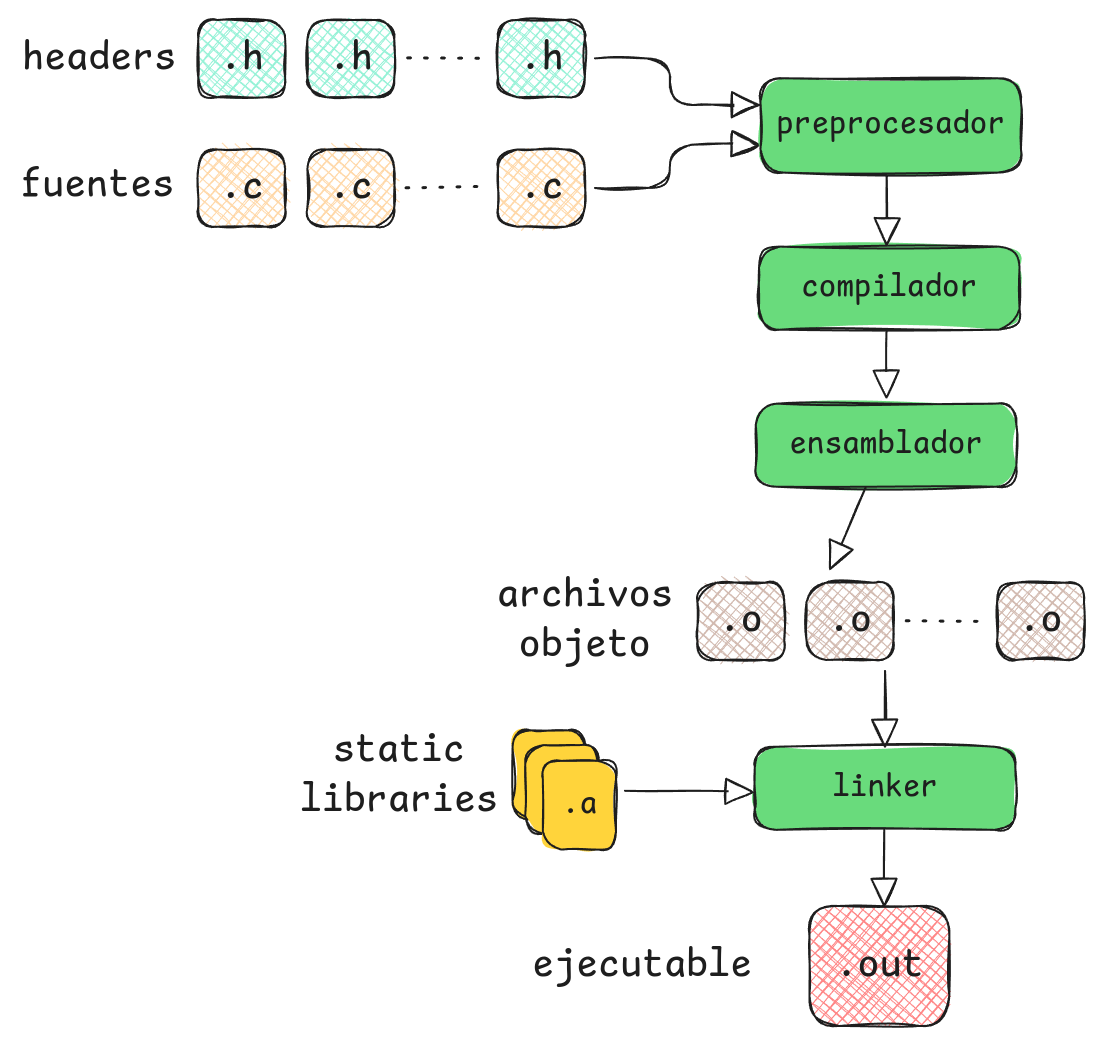
\includegraphics[scale=0.5]{./img/compilacion.png}
  
  \captionof{table}{Compilación en C}
  \label{fig:compilacion}
\end{center}



\subsection*{Header files}

Existe una convención en C de separar la declaración de las definiciones. Las definiciones se ponen en un archivo fuente (\hl{.c}) y las declaraciones en un archivo de cabecera (\hl{.h}). Esto se hace para separar la interfaz de la implementación. La interfaz es lo que el usuario de la biblioteca ve, y la implementación es cómo se hace. Todo lo que necesita el compilador para compilar un archivo fuente es la declaración de las funciones y las variables globales (la interface). Por lo tanto, se incluyen los archivos de cabecera en los archivos fuente. Luego, será el linker el que se encargue de resolver las referencias a las definiciones y verificar que efectivamente, todo lo declarado tenga una definición (y sólo una) en algún lugar. Los errores más comunes que arroja el linker son: \textit{multiple definition} (definición múltiple) y \textit{undefined reference} (referencia indefinida). El primero se da cuando existe más de una definición de una función o variable. El segundo se da cuando no puede encontrar ninguna definición.

\subsubsection*{Compilación separada. Primer ejemplo}
Veamos un ejemplo sencillo de compilación separada:

\begin{cbox}[]{funca.h}
  /* funca.h */
  #ifndef FUNCA_H
  #define FUNCA_H
  
  void a();
  
  #endif // FUNCA_H

\end{cbox}

En este archivo \hl{funca.h} se declara la función \hl{a}. La directiva \hl{\#ifndef} es una directiva de preprocesador que se lee como \textit{if not defined}. Si la macro \hl{FUNCA\_H} no está definida, se define y se incluye el contenido del archivo. Si ya está definida, no se incluye el contenido del archivo. Esto se hace para evitar la inclusión múltiple de un archivo de cabecera en una misma unidad de traducción. Esto puede traer problemas en inclusiones recursivas (A incluye a B, B incluye a C, C incluye a A) y también para incrementar la velocidad de compilación. 

Nuestro archivo fuente sería el siguiente:

\begin{cbox}[]{funca.c}
  /* funca.c */
  #include "funca.h"
  #include <stdio.h>

  void a(){
    printf("Hola, soy A!\n");
  }
\end{cbox}

Y el archivo principal sería:

\begin{cbox}[]{main.c}
  /* main.c */
  #include "funca.h"
  
  int main(){
    a();
  }
\end{cbox}

Para compilar, sería:

\begin{bashbox}
$ gcc -c funca.c -o funca.o
$ gcc -c main.c -o main.o
$ gcc funca.o main.o -o binario
$ ./binario
Hola, soy A!
\end{bashbox}

\subsubsection*{Compilación separada. Segundo ejemplo}

Ahora veamos un ejemplo con 3 archivos fuente y 2 archivos de cabecera.

\begin{cbox}[]{funca.h}
  /* funca.h */
  #ifndef FUNCA_H
  #define FUNCA_H
  
  void a();
  
  #endif // FUNCA_H

\end{cbox}

\begin{cbox}[]{funcb.h}
  /* funcb.h */
  #ifndef FUNCB_H
  #define FUNCB_H
  
  void b();
  
  #endif // FUNCB_H

\end{cbox}

\begin{cbox}[]{funca.c}
/* funca.c */
#include "funca.h"
#include <stdio.h>

void a(){
  printf("Hola, soy A!\n");
}
\end{cbox}

\begin{cbox}[]{funcb.c}
  /* funcb.c */
  #include "funcb.h"
  #include <stdio.h>
  
  void b(){
    printf("Hola, soy B!\n");
  }
\end{cbox}

\begin{cbox}[]{main.c}
  /* main.c */
  #include "funca.h"
  #include "funcb.h"
  
  int main(){
    a();
    b();
  }
\end{cbox}

Para compilar, sería:

\bashinput{snippets/compilation.bash}

Este es un buen momento para ver cómo se actualizaría el \hl{Makefile} para compilar varios archivos. Un primer intento podría ser:

\bashinput[minted language=make]{snippets/make_several_files.bash}

Sin embargo, vemos que las reglas para compilar los archivos \hl{main.o}, \hl{funca.o} y \hl{funcb.o} son iguales. Podemos usar un patrón para definir una regla genérica. Esto se hace con el símbolo \hl{\%}. El símbolo \hl{\%} es un comodín que representa cualquier cadena de caracteres. Por lo tanto, podemos definir una regla genérica para compilar cualquier archivo fuente en un archivo objeto. Este tipo de regla se llama \textit{pattern rule}. Más info en \url{https://www.gnu.org/software/make/manual/html_node/Pattern-Rules.html}.

Por otro lado, como los nombres de los archivos fuentes generan archivos objetos con el mismo nombre, también podemos usar una variable para definir el nombre de los archivos fuentes. Luego, con una \textit{substitution reference} podemos generar los nombres de los archivos objetos. Esto se hace en la línea \hl{OBJ = \$(SRC:.c=.o)}. Esta línea le dice a \texttt{make} que genere una lista de archivos objetos a partir de la lista de archivos fuentes. Más información en \url{https://www.gnu.org/software/make/manual/html_node/Substitution-Refs.html}.

\bashinput[minted language=make]{snippets/make_pattern.bash}

Bueno, esto ya luce bastante bien. Pero falta algo. Ahora tenemos headers. Al ser modificados, es necesario disparar el proceso de compilación de todos los archivos que incluyen a dichos headers. Pero como los archivos \hl{.c} en sí no cambian al modificar los headers, \texttt{make} no los recompila. 

Las dependencias que un módulo \hl{.c} puede tener con los headers \hl{.h} pueden ser complicadas de escribir y mantener a mano. Básicamente, tendríamos que poner todos los \hl{.h} que en caso de ser modificados, necesitan disparar una recompilación del módulo. Esto se haría por ejemplo de la siguiente manera:
\begin{bashbox}[minted language=make]
  module1.o: module1.c module1.h
  module2.o: module2.c module2.h
  module3.o: module3.c module3.h
  main.o: main.c module1.h module2.h
\end{bashbox}

Esto es un problema, porque si tenemos muchos módulos y muchos headers, se hace muy difícil mantenerlo. Además, si un header incluye a otro header, y este último cambia, el primero también debería recompilarse. Pero no lo sabemos a menos que mantengamos el árbol de dependencias a mano. Los include guards justamente evitan duplicaciones en los include, pero cuando tenemos que saber quién incluye a quién y tenemos que además mantener el árbol de dependencias a mano, nos estamos plantando bombas en el camino. Por eso existen unos flags de compilación que se le pueden pasar a gcc: \hl{-MMD -MP}. Esto hace que genere unos archivos de dependencias con extensión \hl{.d}. Se pueden chusmear, porque se van a  generar en el directorio de trabajo. 
Ya que el compilador estudia todas las dependencias entre los archivos, como parte de su proceso de compilación habitual, incluyendo este flag le decimos que nos genere targets armados de Makefile que ya nos sirvan. Es un ejemplo de cooperación entre el compilador y make. Finalmente, lo que hacemos con el último \hl{-include} es justamente "pegar" esas reglas para informarle a make que tenga en cuenta esas dependencias y dispare la compilación en caso de cambios en los headers. El \hl{-include} le dice a make que incluya el archivo de dependencias, pero no arroje un error si no existe. Alta black magic.

\begin{center}
  
\includegraphics[scale=0.5]{./img/drop_makefile.png}
\end{center}

\bashinput[minted language=make]{snippets/make_headers.bash}

\begin{exbox}
  Compilar con ese Makefile y ver qué pasa. Modificar un header y ver qué sucede. 
\end{exbox}

\subsection*{Resolución de variables globales}

En C, las variables globales son visibles en todos los archivos fuente. Por lo tanto, si se define una variable global en un archivo fuente, esta es visible en todos los archivos fuente. Si se define una variable global en un archivo fuente y se declara en otro, el linker se encarga de resolver esta referencia. 

Analicemos el siguiente ejemplo:

\begin{cbox}[]{}
  // file1.h
  #ifndef FILE1_H
  #define FILE1_H

  #include <stdio.h>
  #include "file1.h"

  int count;
  void print_count();

  #endif // FILE1_H
\end{cbox}

\begin{cbox}[]{}
  // file1.c
  #include "file1.h"

  void print_count(){
    printf("Count: %d\n", count);
  }
\end{cbox}

El archivo principal sería:

\begin{cbox}[]{}
  // main.c
  #include <stdio.h>
  #include "file1.h"

  void increment_count() {
    count++;
  }
  
  int main() {
    count = 10;
    print_count();
    increment_count();
    printf("Count en main: %d\n", count);
    return 0;
  }
\end{cbox}

Esto parece tener mucho sentido. ¿Qué sucede si intentamos compilarlo?

\bashinput{snippets/multipledef.bash}

¡Changos! ¿Qué pasó? El linker nos está diciendo que hay una definición múltiple de la variable \hl{count}. Esto es porque la variable \hl{count} está definida en el archivo fuente \hl{file1.c} y en el archivo fuente \hl{main.c}. Para resolver esto, se puede usar la palabra clave \hl{extern} en la declaración de la variable \hl{count} en el header \hl{file1.h}.
\begin{cbox}[]{}
  // file1.h
  #ifndef FILE1_H
  #define FILE1_H

  #include <stdio.h>
  #include "file1.h"
  
  // declaración de la variable count como extern. Esto no es una definición!
  extern int count; 

  void print_count();

  #endif // FILE1_H
\end{cbox}

Necesitamos una definición (ODR) de la variable \hl{count}. Esto se hace en un solo archivo fuente. En este caso, lo hacemos en \hl{main.c}.

\begin{cbox}[]{}
  // main.c
  #include <stdio.h>
  #include "file1.h"

  int count; // definición de la variable count

  void increment_count() {
    count++;
  }
  
  int main() {
    count = 10;
    print_count();
    increment_count();
    printf("Count en main: %d\n", count);
    return 0;
  }
\end{cbox}

Compilamos:

\begin{bashbox}
$ gcc -Wall -c file1.c -o file1.o
$ gcc -Wall -c main.c -o main.o
$ gcc -Wall file1.o main.o -o binario
$ ./binario
Count: 10
Count en main: 11
\end{bashbox}


\newpage
\section*{Referencias}

\epigraph{\textit{Muad'Dib learned rapidly because his first training was in how to learn. And the first lesson of all was the basic trust that he could learn. It's shocking to find how many people do not believe they can learn, and how many more believe learning to be difficult.}}

\begin{itemize}
  \item Kernighan, Ritchie - The C Programming Language, 2nd Edition.
  \item Seacord, Robert - Effective C: An Introduction to Professional C Programming 
  \item C reference: \url{https://en.cppreference.com/w/c }
  \item GNU C reference: \url{https://gcc.gnu.org/onlinedocs/gcc/}
  \item GNU Make reference: \url{https://www.gnu.org/software/make/manual/html_node/}
\end{itemize}


\end{document}
